% EGE 2027, task 5. Source IDs and URLs are kept in comments.
% Editable task bank. Append new BankTask blocks at the end of the document.
\documentclass[12pt,a4paper]{article}
\usepackage{physics-textbook}
\usepackage{graphicx,needspace}
\newif\ifShowSolutions
\ifdefined\TutorEdition
  \ShowSolutionstrue
\else
  \ShowSolutionsfalse
\fi
\newcounter{banktask}
\newcommand{\BankTask}[3]{%
  \refstepcounter{banktask}%
  \Needspace{35mm}\par\medskip\noindent\begin{minipage}{\linewidth}%
  \noindent\textbf{\thebanktask.}\quad #2\par
  \ifShowSolutions
    #3\par
    \ifdefined\TutorEdition
      \ifcsname TutorSource#1\endcsname
        \smallskip{\small\csname TutorSource#1\endcsname\par}%
      \fi
    \fi
  \fi
  \end{minipage}\par\medskip
}
\begin{document}
$g=10\,\text{м}/\text{с}^2$.



% Source eeB001: https://ege.fipi.ru/bank/questions.php?search=1&proj=BA1F39653304A5B041B656915DC36B38&qid=eeB001
\BankTask{eeB001}{
В таблице представлены данные о положении грузика, прикреплённого к пружине и совершающего гармонические колебания вдоль горизонтальной оси $Ox$, в различные моменты времени.
\begin{center}{\small\setlength{\tabcolsep}{3pt}\begin{tabular}{|c|c|c|c|c|c|c|c|c|c|c|c|c|c|c|c|c|}\hline $t,\,\text{с}$ & $0{,}0$ & $0{,}1$ & $0{,}2$ & $0{,}3$ & $0{,}4$ & $0{,}5$ & $0{,}6$ & $0{,}7$ & $0{,}8$ & $0{,}9$ & $1{,}0$ & $1{,}1$ & $1{,}2$ & $1{,}3$ & $1{,}4$ & $1{,}5$ \\\hline $x,\,\text{мм}$ & $0$ & $2{,}5$ & $4{,}5$ & $6{,}0$ & $7{,}0$ & $7{,}5$ & $7{,}0$ & $6{,}0$ & $4{,}5$ & $2{,}5$ & $0$ & $-2{,}5$ & $-4{,}5$ & $-6{,}0$ & $-7{,}0$ & $-7{,}5$ \\\hline\end{tabular}}\end{center}
\begin{enumerate}
\item Период колебаний грузика равен $1\,\text{с}$.
\item Амплитуда колебаний грузика равна $15\,\text{мм}$.
\item Потенциальная энергия пружины маятника в момент времени $1{,}5\,\text{с}$ минимальна.
\item Кинетическая энергия грузика в момент времени $1{,}0\,\text{с}$ максимальна.
\item Модуль ускорения грузика в момент времени $1{,}5\,\text{с}$ максимален.
\end{enumerate}
}{
\smallskip\noindent\textbf{Решение от GPT}\par
Из таблицы $A=7{,}5\,\text{мм}$, $T=2\,\text{с}$. При $t=1{,}0\,\text{с}$ $x=0$, поэтому кинетическая энергия максимальна; при $t=1{,}5\,\text{с}$ $|x|=A$, поэтому $|a|=\omega^2A$ максимально. Ответ: $45$.
}

% Source A7Be77: https://ege.fipi.ru/bank/questions.php?search=1&proj=BA1F39653304A5B041B656915DC36B38&qid=A7Be77
\BankTask{A7Be77}{
В лабораторной работе изучали движение небольшого бруска массой $200\,\text{г}$ по горизонтальной шероховатой поверхности под действием горизонтальной постоянной силы, равной по модулю $800\,\text{мН}$. Зависимость модуля скорости бруска от времени приведена в таблице.
\begin{center}{\small\setlength{\tabcolsep}{3pt}\begin{tabular}{|c|c|c|c|c|c|c|c|}\hline $t,\,\text{с}$ & $0$ & $0{,}1$ & $0{,}2$ & $0{,}3$ & $0{,}4$ & $0{,}5$ & $0{,}6$ \\\hline $u,\,\text{м}/\text{с}$ & $0$ & $0{,}2$ & $0{,}4$ & $0{,}6$ & $0{,}8$ & $1{,}0$ & $1{,}2$ \\\hline\end{tabular}}\end{center}
\begin{enumerate}
\item Брусок движется равномерно.
\item Модуль ускорения бруска равен $0{,}4\,\text{м}/\text{с}^{2}$.
\item Модуль равнодействующей сил, действующих на брусок, равен $0{,}4\,\text{Н}$.
\item Коэффициент трения бруска о поверхность $\mu=$ $0{,}3$.
\item В момент времени $0{,}3\,\text{с}$ кинетическая энергия бруска равна $36\,\text{мДж}$.
\end{enumerate}
}{
\smallskip\noindent\textbf{Решение от GPT}\par
$a=0{,}2/0{,}1=2\,\text{м}/\text{с}^2$, $F_{\text{рез}}=ma=0{,}4\,\text{Н}$. Трение $F_{\text{тр}}=0{,}8-0{,}4=0{,}4\,\text{Н}$, $\mu=0{,}4/(0{,}2\cdot10)=0{,}2$. При $t=0{,}3\,\text{с}$ $E_{\text{к}}=0{,}2\cdot0{,}6^2/2=0{,}036\,\text{Дж}=36\,\text{мДж}$. Ответ: $35$.
}

% Source 9F061F: https://ege.fipi.ru/bank/questions.php?search=1&proj=BA1F39653304A5B041B656915DC36B38&qid=9F061F
\BankTask{9F061F}{
Тело совершает гармонические колебания вдоль оси $Ox$. В таблице приведены координаты этого тела через равные промежутки времени.
\begin{center}{\small\setlength{\tabcolsep}{3pt}\begin{tabular}{|c|c|c|c|c|c|c|c|}\hline $t,\,\text{с}$ & $0$ & $0{,}2$ & $0{,}4$ & $0{,}6$ & $0{,}8$ & $1{,}0$ & $1{,}2$ \\\hline $x,\,\text{см}$ & $0$ & $2$ & $4$ & $2$ & $0$ & $2$ & $4$ \\\hline\end{tabular}}\end{center}
\begin{enumerate}
\item Амплитуда колебаний тела равна $8\,\text{см}$.
\item Частота колебаний тела равна $1{,}25\,\text{Гц}$.
\item Модуль ускорения тела максимален в момент времени $0{,}2\,\text{с}$.
\item В момент времени $0{,}4\,\text{с}$ тело проходит положение равновесия.
\item В момент времени $0{,}6\,\text{с}$ тело обладает максимальной кинетической энергией.
\end{enumerate}
}{
\smallskip\noindent\textbf{Решение от GPT}\par
Положение равновесия $x_{\text{равн}}=2\,\text{см}$, амплитуда $A=2\,\text{см}$, период $T=0{,}8\,\text{с}$; $\nu=1/T=1{,}25\,\text{Гц}$. В момент $0{,}6\,\text{с}$ тело в равновесии и его кинетическая энергия максимальна. Ответ: $25$.
}

% Source 12C0AE: https://ege.fipi.ru/bank/questions.php?search=1&proj=BA1F39653304A5B041B656915DC36B38&qid=12C0AE
\BankTask{12C0AE}{
Небольшой груз массой $0{,}1\,\text{кг}$ подвешен на невесомой нерастяжимой нити длиной $40\,\text{см}$. В результате толчка груз стал совершать незатухающие колебания в вертикальной плоскости. В таблице приведена зависимость от времени $t$ для высоты $h$ подъёма груза относительно положения равновесия.
\begin{center}{\small\setlength{\tabcolsep}{3pt}\begin{tabular}{|c|c|c|c|c|c|c|c|c|c|}\hline $t,\,\text{с}$ & $0$ & $0{,}2$ & $0{,}4$ & $0{,}6$ & $0{,}8$ & $1{,}0$ & $1{,}2$ & $1{,}4$ & $1{,}6$ \\\hline $h,\,\text{см}$ & $0$ & $12$ & $20$ & $12$ & $0$ & $12$ & $20$ & $12$ & $0$ \\\hline\end{tabular}}\end{center}
\begin{enumerate}
\item Период колебаний груза равен $0{,}8\,\text{с}$.
\item В момент времени $0{,}4\,\text{с}$ скорость груза максимальна.
\item В промежуток времени от $0{,}2$ до $1{,}0\,\text{с}$ кинетическая энергия груза достигла минимального значения $2$ раза.
\item В момент $1{,}2\,\text{с}$ кинетическая энергия груза равна $0$.
\item Максимальная скорость груза равна $2\,\text{м}/\text{с}$.
\end{enumerate}
}{
\smallskip\noindent\textbf{Решение от GPT}\par
При $t=1{,}2\,\text{с}$ груз на максимальной высоте, поэтому $E_{\text{к}}=0$. Из сохранения энергии $mv_{\max}^2/2=mgh_{\max}$: $v_{\max}=\sqrt{2\cdot10\cdot0{,}2}=2\,\text{м}/\text{с}$. Высота повторяется через полпериода, поэтому $T=1{,}6\,\text{с}$; на интервале $0{,}2\! -\!1{,}0\,\text{с}$ минимум кинетической энергии один. Ответ: $45$.
}

% Source ADDAE8: https://ege.fipi.ru/bank/questions.php?search=1&proj=BA1F39653304A5B041B656915DC36B38&qid=ADDAE8
\BankTask{ADDAE8}{
Тело брошено вертикально вверх с поверхности Земли в момент времени $t=0$. В таблице приведены результаты измерения модуля скорости тела в зависимости от времени.
\begin{center}{\small\setlength{\tabcolsep}{3pt}\begin{tabular}{|c|c|c|c|c|c|c|c|c|c|c|}\hline $t,\,\text{с}$ & $0{,}1$ & $0{,}2$ & $0{,}3$ & $0{,}4$ & $0{,}5$ & $0{,}6$ & $0{,}7$ & $0{,}8$ & $0{,}9$ & $1{,}0$ \\\hline $|v|,\,\text{м}/\text{с}$ & $4{,}0$ & $3{,}0$ & $2{,}0$ & $1{,}0$ & $0$ & $1{,}0$ & $2{,}0$ & $3{,}0$ & $4{,}0$ & $5{,}0$ \\\hline\end{tabular}}\end{center}
\begin{enumerate}
\item Тело поднялось на максимальную высоту, равную $0{,}8\,\text{м}$.
\item На высоте $0{,}8\,\text{м}$ от поверхности Земли скорость тела была равна $3{,}0\,\text{м}/\text{с}$.
\item Начальная скорость тела была равна $4\,\text{м}/\text{с}$.
\item В момент времени $t=0{,}9\,\text{с}$ тело находилось на высоте $0{,}45\,\text{м}$ от поверхности Земли.
\item В момент времени $t=0{,}2\,\text{с}$ тело находилось на высоте $0{,}45\,\text{м}$ от поверхности Земли.
\end{enumerate}
}{
\smallskip\noindent\textbf{Решение от GPT}\par
По таблице $g=10\,\text{м}/\text{с}^2$, $v_0=5\,\text{м}/\text{с}$. Высота $h=5t-5t^2$, $h_{\max}=1{,}25\,\text{м}$. На высоте $0{,}8\,\text{м}$ $v^2=v_0^2-2gh=9$, то есть $|v|=3\,\text{м}/\text{с}$. При $t=0{,}9\,\text{с}$ $h=4{,}5-4{,}05=0{,}45\,\text{м}$; при $0{,}2\,\text{с}$ $h=0{,}8\,\text{м}$. Ответ: $24$.
}

% Source 9D2AE0: https://ege.fipi.ru/bank/questions.php?search=1&proj=BA1F39653304A5B041B656915DC36B38&qid=9D2AE0
\BankTask{9D2AE0}{
В лаборатории исследовали прямолинейное движение тела массой $m=300\,\text{г}$ из состояния покоя. В таблице приведена экспериментально полученная зависимость пути, пройденного телом, от времени.
\begin{center}{\small\setlength{\tabcolsep}{3pt}\begin{tabular}{|c|c|c|c|c|c|c|c|c|}\hline $t,\,\text{с}$ & $0$ & $1$ & $2$ & $3$ & $4$ & $5$ & $6$ & $7$ \\\hline $L,\,\text{м}$ & $0$ & $1$ & $4$ & $9$ & $16$ & $25$ & $36$ & $49$ \\\hline\end{tabular}}\end{center}
\begin{enumerate}
\item Тело двигалось равноускоренно.
\item Скорость тела в момент времени $4\,\text{с}$ равнялась $8\,\text{м}/\text{с}$.
\item Кинетическая энергия тела в момент времени $5\,\text{с}$ равна $25\,\text{Дж}$.
\item Равнодействующая сил, действующих на тело, всё время возрастала.
\item За первые $3\,\text{с}$ работа равнодействующей сил, действующих на тело, была равна $5{,}4\,\text{Дж}$.
\end{enumerate}
}{
\smallskip\noindent\textbf{Решение от GPT}\par
По данным $L=t^2=at^2/2$, значит $a=2\,\text{м}/\text{с}^2$ и $v=2t$. При $t=4\,\text{с}$ $v=8\,\text{м}/\text{с}$; сила $ma=0{,}6\,\text{Н}$ постоянна. При $t=5\,\text{с}$ $E_{\text{к}}=15\,\text{Дж}$. Работа за первые $3\,\text{с}$ $A=\Delta E_{\text{к}}=0{,}3\cdot6^2/2=5{,}4\,\text{Дж}$. Ответ: $125$.
}

% Source 3A9974: https://ege.fipi.ru/bank/questions.php?search=1&proj=BA1F39653304A5B041B656915DC36B38&qid=3A9974
\BankTask{3A9974}{
Грузовик массой $10\,\text{т}$ проезжает верхнюю точку выпуклого моста, радиус кривизны которого равен $80\,\text{м}$, двигаясь равномерно со скоростью $72\,\text{км}/\text{ч}$.
\begin{enumerate}
\item Сила тяжести, действующая на грузовик, равна $10\,\text{кН}$.
\item Сумма сил, действующих на грузовик, направлена вертикально вверх и перпендикулярна его скорости.
\item Центростремительное ускорение грузовика равно $5\,\text{м}/\text{с}^{2}$.
\item Сила, с которой мост действует на грузовик, меньше $40\,\text{кН}$ и направлена вертикально вверх.
\item Сила, с которой грузовик действует на мост, направлена вертикально вниз и равна $50\,\text{кН}$.
\end{enumerate}
}{
\smallskip\noindent\textbf{Решение от GPT}\par
$m=10^4\,\text{кг}$, $v=20\,\text{м}/\text{с}$. Ускорение $a=v^2/R=5\,\text{м}/\text{с}^2$ направлено вниз. $mg=100\,\text{кН}$, $N=m(g-a)=50\,\text{кН}$ направлена вверх; на мост грузовик действует вниз с той же силой. Ответ: $35$.
}

% Source F64C40: https://ege.fipi.ru/bank/questions.php?search=1&proj=BA1F39653304A5B041B656915DC36B38&qid=F64C40
\BankTask{F64C40}{
Искусственный спутник обращается вокруг Земли по вытянутой эллиптической орбите. В некоторый момент времени спутник проходит точку минимального удаления от Земли.
\begin{enumerate}
\item Кинетическая энергия спутника при прохождении этого положения максимальна.
\item Сила притяжения спутника к Земле в этом положении максимальна.
\item Полная механическая энергия спутника в этом положении достигает максимума.
\item Скорость спутника при прохождении этого положения минимальна.
\item Ускорение спутника при прохождении этого положения равно $0$.
\end{enumerate}
}{
\smallskip\noindent\textbf{Решение от GPT}\par
В перигее $r$ минимален, поэтому $F=GMm/r^2$ максимальна. Полная энергия постоянна; потенциальная $-GMm/r$ минимальна, следовательно, кинетическая энергия и скорость максимальны. Ответ: $12$.
}

% Source 7D140C: https://ege.fipi.ru/bank/questions.php?search=1&proj=BA1F39653304A5B041B656915DC36B38&qid=7D140C
\BankTask{7D140C}{
Мальчик поднимает вверх гирю массой $10\,\text{кг}$, действуя на неё постоянной силой $120\,\text{Н}$, направленной вертикально вверх.
\begin{enumerate}
\item Вес гири равен $120\,\text{Н}$ и направлен вверх.
\item Гиря действует на руку мальчика с силой $100\,\text{Н}$, направленной вниз.
\item Равнодействующая сил, действующих на гирю, равна $240\,\text{Н}$ и направлена вверх.
\item Ускорение гири равно $2\,\text{м}/\text{с}^{2}$.
\item Если мальчик приложит к гире направленную вертикально силу $90\,\text{Н}$, он не сможет её поднять.
\end{enumerate}
}{
\smallskip\noindent\textbf{Решение от GPT}\par
$mg=100\,\text{Н}$, $F_{\text{рез}}=120-100=20\,\text{Н}$ вверх, $a=20/10=2\,\text{м}/\text{с}^2$. Гиря действует на руку вниз с силой $120\,\text{Н}$. Сила $90\,\text{Н}<mg$ не позволяет поднять гирю из покоя. Ответ: $45$.
}

% Source ACFD5A: https://ege.fipi.ru/bank/questions.php?search=1&proj=BA1F39653304A5B041B656915DC36B38&qid=ACFD5A
\BankTask{ACFD5A}{
Искусственный спутник обращается вокруг Земли по вытянутой эллиптической орбите. В некоторый момент времени спутник проходит положение максимального удаления от Земли.
\begin{enumerate}
\item Скорость спутника при прохождении этого положения максимальна.
\item Сила притяжения спутника к Земле при прохождении этого положения максимальна.
\item Полная механическая энергия спутника при прохождении этого положения максимальна.
\item Импульс спутника при прохождении этого положения минимален.
\item Ускорение спутника при прохождении этого положения минимально.
\end{enumerate}
}{
\smallskip\noindent\textbf{Решение от GPT}\par
В апогее $r$ максимален; поэтому $F=GMm/r^2$ и $a=GM/r^2$ минимальны. Полная механическая энергия постоянна, потенциальная максимальна, значит скорость и импульс минимальны. Ответ: $45$.
}

% Source D82e7B: https://ege.fipi.ru/bank/questions.php?search=1&proj=BA1F39653304A5B041B656915DC36B38&qid=D82e7B
\BankTask{D82e7B}{
Два тела, каждое массой $2\,\text{кг}$, движутся на одной прямой, вдоль которой направлена ось $O x$ На рисунке приведены графики зависимости проекций $\upsilon_x$ их скорости от времени $t.$
\begin{center}\begin{tikzpicture}[x=.225cm,y=.45cm,>=stealth]
\draw[thin,dashed,xstep=2,ystep=1] (0,0) grid (20,8);
\draw[->] (0,0)--(22,0) node[right] {$t,\,\text{с}$};
\draw[->] (0,0)--(0,9) node[above] {$\upsilon_x,\,\text{м}/\text{с}$};
\foreach \x in {0,4,8,12,16} \node[below] at (\x,0) {$\x$};
\foreach \y in {2,4,6} \node[left] at (0,\y) {$\y$};
\draw[very thick] (0,7)--(20,{19/7}); \node at (6,6.8) {$1$};
\draw[very thick] (0,.5)--(20,5.5); \node at (8,1.7) {$2$};
\end{tikzpicture}\end{center}
\begin{enumerate}
\item Равнодействующая сил, действующих на тело $1$, остаётся постоянной в течение всего времени наблюдения.
\item В промежутке времени от $0$ до $14\,\text{с}$ тела двигались навстречу друг другу.
\item Путь, пройденный телом $1$ за промежуток времени от $0$ до $18\,\text{с}$, больше пути, пройденного телом $2$ за тот же промежуток времени.
\item Кинетическая энергия тела $2$ за промежуток времени от $6$ до $14\,\text{с}$ увеличилась в $2$ раза.
\item Модуль импульса тела $2$ в момент времени $t=10\,\text{с}$ равен $10\,\text{кг}\cdot\text{м}/\text{с}$.
\end{enumerate}
}{
\smallskip\noindent\textbf{Решение от GPT}\par
Линейные графики задают $v_{1x}=7-\frac{3}{14}t$ и $v_{2x}=0{,}5+0{,}25t$ в СИ. Равнодействующая на тело $1$ постоянна; обе скорости положительны. За первые $18\,\text{с}$ пути $s_1=7\cdot18-\frac{3}{28}\cdot18^2=\frac{639}{7}\,\text{м}\approx91{,}3\,\text{м}$ и $s_2=(0{,}5+5)18/2=49{,}5\,\text{м}$, значит $s_1>s_2$. Для тела $2$ $E_{\text{к}}(14)/E_{\text{к}}(6)=(4/2)^2=4$, $p(10)=2\cdot3=6\,\text{кг}\cdot\text{м}/\text{с}$. Ответ: $13$.
}

% Source B2D13F: https://ege.fipi.ru/bank/questions.php?search=1&proj=BA1F39653304A5B041B656915DC36B38&qid=B2D13F
\BankTask{B2D13F}{
На рисунке представлены графики зависимости давления $p$ от глубины погружения $h$ для двух покоящихся жидкостей: воды и лёгкой жидкости эфира (плотность эфира $\rho_{\text{э}}=0{,}72\,\text{г}/\text{см}^{3}$), при постоянной температуре.
\begin{center}\begin{tikzpicture}[x=.17cm,y=.009cm,>=stealth]
\draw[thin,black!65,xstep=2.5,ystep=25] (0,0) grid (30,450);
\draw[->] (0,0)--(33,0) node[right] {$h,\,\text{м}$};
\draw[->] (0,0)--(0,480) node[above] {$p,\,\text{кПа}$};
\foreach \x in {0,5,10,15,20,25,30} \node[below] at (\x,0) {$\x$};
\foreach \y in {50,100,150,200,250,300,350,400,450} \node[left] at (0,\y) {$\y$};
\draw[very thick] (0,100)--(30,400);\node at (22,355) {вода};
\draw[very thick] (0,100)--(30,310);\node at (24,240) {эфир};
\end{tikzpicture}\end{center}
\begin{enumerate}
\item С глубиной погружения давление в воде возрастает быстрее.
\item В воде давление возрастёт вдвое на глубине $20\,\text{м}$.
\item Плотность оливкового масла $0{,}92\,\text{г}/\text{см}^{3}$, график аналогичной зависимости давления от глубины для масла окажется между зависимостью для эфира и осью абсцисс.
\item По мере подъёма из воды давление падает до нуля.
\item Плотность ртути $13{,}59\,\text{г}/\text{см}^{3}$, график аналогичной зависимости давления от глубины для ртути окажется между зависимостью для воды и осью ординат (вертикальной осью).
\end{enumerate}
}{
\smallskip\noindent\textbf{Решение от GPT}\par
$p=p_0+\rho gh$; большему $\rho$ отвечает больший наклон. Поэтому вода даёт более крутой график, чем эфир, а ртуть --- более крутой, чем вода. Для масла $\rho_{\text{э}}<\rho_{\text{м}}<\rho_{\text{в}}$, поэтому его график между графиками эфира и воды. На поверхности $p=p_0=100\,\text{кПа}\ne0$; при $h=20\,\text{м}$ $p=300\,\text{кПа}$, а не $200$. Ответ: $15$.
}

% Source B29D40: https://ege.fipi.ru/bank/questions.php?search=1&proj=BA1F39653304A5B041B656915DC36B38&qid=B29D40
\BankTask{B29D40}{
Изучая на практике закон Архимеда, учащиеся опускали цилиндр объёмом $V=10\,\text{см}^3$ в различные жидкости (см. таблицу) и измеряли объём цилиндра, погружённый в жидкость. По результатам измерений была построена обобщённая зависимость объёма погружённой части цилиндра $V_{\text{погр}}$ от плотности жидкости $\rho$ (см. рисунок).
\begin{center}{\small\setlength{\tabcolsep}{2pt}\begin{tabular}{|c|c|c|c|c|c|c|c|}\hline Жидкость & Бензин & Спирт & Вода & Глицерин & Хлороформ & Бромоформ & Дийодметан \\\hline $\rho,\,\text{г}/\text{см}^3$ & $0{,}71$ & $0{,}79$ & $1{,}0$ & $1{,}26$ & $1{,}49$ & $2{,}89$ & $3{,}25$ \\\hline\end{tabular}}\end{center}
\begin{center}\begin{tikzpicture}[x=1.2cm,y=.44cm,>=stealth]
\draw[thin,black!65,xstep=.25,ystep=1] (0,0) grid (4,10);
\foreach \q in {0,.25,...,4} \draw (\q,.08)--(\q,-.08);
\foreach \q in {0,.5,...,10} \draw (.035,\q)--(-.035,\q);
\draw[->] (0,0)--(4.6,0) node[right] {$\rho,\,\text{г}/\text{см}^3$};
\draw[->] (0,0)--(0,11.2) node[above] {$V_{\text{погр}},\,\text{см}^3$};
\foreach \x/\lab in {.5/{0{,}5},1/{1{,}0},1.5/{1{,}5},2/{2{,}0},2.5/{2{,}5},3/{3{,}0},3.5/{3{,}5},4/{4{,}0}} \node[below] at (\x,0) {$\lab$};
\node[below left] at (0,0) {$0$};
\foreach \y in {1,2,3,4,5,6,7,8,9,10} \node[left] at (0,\y) {$\y$};
\draw[very thick] (0,10)--(1,10);
\draw[very thick,domain=1:4,samples=60] plot (\x,{10/\x});
\end{tikzpicture}\end{center}
\begin{enumerate}
\item Цилиндр плавает в бромоформе
\item Цилиндр тонет в глицерине
\item При возрастании плотности жидкостей до $1\,\text{г}/\text{см}^{3}$ сила Архимеда, действующая на цилиндр, опущенный в жидкость, возрастает.
\item При возрастании плотности жидкости от $1{,}5$ до $3{,}25\,\text{г}/\text{см}^{3}$ сила Архимеда убывает
\item На цилиндр, плавающий в глицерине, действует выталкивающая сила, составляющая около $80\,\text{мН}$
\end{enumerate}
}{
\smallskip\noindent\textbf{Решение от GPT}\par
Граница плавания соответствует $\rho=1\,\text{г}/\text{см}^3$, значит плотность цилиндра $1\,\text{г}/\text{см}^3$, масса $10\,\text{г}$. В бромоформе он плавает. При $\rho\leq1\,\text{г}/\text{см}^3$ тело погружено полностью и $F_A=\rho gV$ растёт. Далее при плавании $F_A=mg=0{,}1\,\text{Н}=100\,\text{мН}$ постоянна. Ответ: $13$.
}

% Source 8c1642: https://ege.fipi.ru/bank/questions.php?search=1&proj=BA1F39653304A5B041B656915DC36B38&qid=8c1642
\BankTask{8c1642}{
На рисунке показан график зависимости координаты $x$ тела, движущегося вдоль оси $Ox$, от времени $t$.
\begin{center}\begin{tikzpicture}[x=1cm,y=.8cm,>=stealth]
\draw[->] (0,0)--(5.4,0) node[right] {$t$};
\draw[->] (0,0)--(0,5.1) node[above] {$x$};
\node[below left] at (0,0) {$0$};
\draw[very thick] (0,1.6) .. controls (.3,1.0) and (.45,.8) .. (.75,.8) .. controls (1.5,.8) and (1.75,2.1) .. (2.5,3.7) .. controls (2.875,4.5) and (3.10546875,4.8) .. (3.45,4.8) .. controls (3.9,4.8) and (4.3,4.0) .. (4.65,3.0) .. controls (4.72,2.8) and (4.8,2.6) .. (4.9,2.3);
\fill (.75,.8) circle (1.5pt) node[below] {$A$};
\fill (2.5,3.7) circle (1.5pt) node[above left] {$B$};
\fill (3.45,4.8) circle (1.5pt) node[above] {$C$};
\fill (4.65,3.0) circle (1.5pt) node[right] {$D$};
\end{tikzpicture}\end{center}
\begin{enumerate}
\item На участке $CD$ модуль скорости тела увеличивается.
\item В точке $A$ проекция ускорения тела на ось $Ox$ отрицательна.
\item На участке $BC$ модуль скорости тела увеличивается.
\item В точке $B$ ускорение тела и его скорость направлены в противоположные стороны.
\item В точке $B$ проекция скорости тела на ось $Ox$ отрицательна.
\end{enumerate}
}{
\smallskip\noindent\textbf{Решение от GPT}\par
На участке $CD$ отрицательный наклон графика по модулю растёт, значит модуль скорости увеличивается. В точке $A$ минимум координаты, кривизна направлена вверх: $a_x>0$. В точке $B$ наклон положителен, но уменьшается при приближении к $C$: $v_x>0$, $a_x<0$. Ответ: $14$.
}

% Source 72e2A7: https://ege.fipi.ru/bank/questions.php?search=1&proj=BA1F39653304A5B041B656915DC36B38&qid=72e2A7
\BankTask{72e2A7}{
На рисунке приведены графики зависимости координаты $x$ от времени $t$ для двух точечных тел $1$ и $2$, движущихся по прямой, вдоль которой направлена ось $Ox$. Масса каждого тела равна $0{,}5\,\text{кг}$.
\begin{center}\begin{tikzpicture}[x=.25cm,y=.5cm,>=stealth]
\draw[thin,black!65,xstep=2,ystep=1] (0,0) grid (20,8);
\draw[->] (0,0)--(22,0) node[right] {$t,\,\text{с}$};
\draw[->] (0,0)--(0,9) node[above] {$x,\,\text{м}$};
\foreach \x in {0,4,8,12,16,20} \node[below] at (\x,0) {$\x$};
\foreach \y in {2,4,6} \node[left] at (0,\y) {$\y$};
\draw[very thick] (0,.5)--(20,5.5);\node at (12,3.9) {$1$};
\draw[very thick,domain=0:19.2,samples=60] plot (\x,{1+(\x-10)^2/16});\node at (17,1.7) {$2$};
\end{tikzpicture}\end{center}
\begin{enumerate}
\item Проекция скорости тела $2$ на ось $Ox$ в момент времени $4\,\text{с}$ отрицательна.
\item Тело $1$ движется со скоростью $3\,\text{м}/\text{с}$.
\item Проекция ускорения тела $2$ на ось $Ox$ отрицательна.
\item Кинетическая энергия тела $1$ в момент времени $10\,\text{с}$ равна $2{,}25\,\text{Дж}$.
\item Расстояние между точками встречи тел равно $3\,\text{м}$.
\end{enumerate}
}{
\smallskip\noindent\textbf{Решение от GPT}\par
При $t=4\,\text{с}$ график тела $2$ убывает, значит $v_{2x}<0$. Скорость тела $1$ равна наклону прямой: $v_1=(5-2)/(18-6)=0{,}25\,\text{м}/\text{с}$, а его энергия $E_{\text{к}1}=0{,}5\cdot0{,}25^2/2\ne2{,}25\,\text{Дж}$. Парабола вогнута вверх, поэтому $a_{2x}>0$. Координаты встреч $x_a=2\,\text{м}$ и $x_b=5\,\text{м}$ отличаются на $3\,\text{м}$. Ответ: $15$.
}

% Source C1C6AE: https://ege.fipi.ru/bank/questions.php?search=1&proj=BA1F39653304A5B041B656915DC36B38&qid=C1C6AE
\BankTask{C1C6AE}{
На рисунке приведены зависимости координат $x$ двух грузов $1$ и $2$ от времени $t$ в процессе их малых колебаний на гладкой горизонтальной плоскости. Грузы имеют одинаковую массу $m$ и прикреплены к пружинам жёсткостью $k_{1}$ (груз $1$) и жёсткостью $k_{2}$ (груз $2$). Колебания груза $1$ обозначены сплошной линией, груза $2$ – пунктиром.
\begin{center}\begin{tikzpicture}[x=.96cm,y=.8cm,>=stealth]
\foreach \q in {0,1,2,3,4,5,6} \draw[thin,black!65] (\q,-2)--(\q,2);
\draw[thin,black!65] (0,2)--(6,2) (0,-2)--(6,-2);
\foreach \h in {-1.5,-1,-.5,.5,1,1.5} \draw[thin,black!65] (0,\h)--(1.1,\h) (1.4,\h)--(2,\h) (2.8,\h)--(3.5,\h) (4,\h)--(5,\h) (5.3,\h)--(6,\h);
\draw[->] (0,0)--(6.6,0) node[right] {$t,\,\text{с}$};
\draw[->] (0,-2)--(0,2.7) node[above] {$x,\,\text{см}$};
\foreach \x in {1,2,3,4,5,6} \node[below] at (\x,0) {$\x$};
\foreach \y in {-2,-1,0,1,2} \node[left] at (0,\y) {$\y$};
\draw[very thick,domain=0:6,samples=100] plot (\x,{2*sin(90*\x)});
\draw[thick,dashed,domain=0:6,samples=100] plot (\x,{cos(90*(\x-.25))});
\node at (5.8,1.85) {$1$};\node at (3.2,1.0) {$2$};
\end{tikzpicture}\end{center}
\begin{enumerate}
\item Периоды колебаний грузов одинаковы.
\item Максимальные потенциальные энергии деформированных пружин одинаковы.
\item Жёсткость пружины $k_{1}$ меньше жёсткости пружины $k_{2}$.
\item Амплитуды колебаний грузов одинаковы.
\item Максимальная кинетическая энергия груза $1$ в четыре раза больше, чем максимальная кинетическая энергия груза $2$.
\end{enumerate}
}{
\smallskip\noindent\textbf{Решение от GPT}\par
По графику периоды одинаковы, значит при одинаковых массах $k_1=k_2$. Амплитуды $A_1=2\,\text{см}$ и $A_2=1\,\text{см}$ различаются вдвое. Поэтому $E_{\text{к max}}=kA^2/2$ у первого груза вчетверо больше. Ответ: $15$.
}

% Source D4E9EE: https://ege.fipi.ru/bank/questions.php?search=1&proj=BA1F39653304A5B041B656915DC36B38&qid=D4E9EE
\BankTask{D4E9EE}{
В инерциальной системе отсчёта вдоль оси $Ox$ движется тело массой $20\,\text{кг}$. На рисунке приведён график зависимости проекции скорости $V_{x}$ этого тела от времени $t$.
\begin{center}
\begin{tikzpicture}[x=0.06cm,y=0.6cm,>=stealth]
\draw[thin,black!65,xstep=10,ystep=1] (0,0) grid (100,4);
\draw[->] (0,0)--(110,0) node[right] {$t,\,\text{с}$};
\draw[->] (0,0)--(0,5) node[above] {$v_x,\,\text{м}/\text{с}$};

\node[below] at (10,0) {$10$};
\node[below] at (20,0) {$20$};
\node[below] at (30,0) {$30$};
\node[below] at (40,0) {$40$};
\node[below] at (50,0) {$50$};
\node[below] at (60,0) {$60$};
\node[below] at (70,0) {$70$};
\node[below] at (80,0) {$80$};
\node[below] at (90,0) {$90$};
\node[below] at (100,0) {$100$};
\node[left] at (0,0) {$0$};
\node[left] at (0,1) {$1$};
\node[left] at (0,2) {$2$};
\node[left] at (0,3) {$3$};
\node[left] at (0,4) {$4$};
\draw[very thick] (0,0)--(20,4)--(60,4)--(80,3)--(100,0);
\end{tikzpicture}
\end{center}
\begin{enumerate}
\item Модуль ускорения тела в промежутке времени от $0$ до $20\,\text{с}$ в два раза больше модуля ускорения тела в промежутке времени от $60$ до $80\,\text{с}$
\item В промежутке времени от $0$ до $10\,\text{с}$ тело переместилось на $20\,\text{м}$
\item В момент времени $40\,\text{с}$ равнодействующая сил, действующих на тело, равна $0$
\item В промежутке времени от $80$ до $100\,\text{с}$ импульс тела уменьшился на $60\,\text{кг}\cdot\text{м}/\text{с}$
\item Кинетическая энергия тела в промежутке времени от $10$ до $20\,\text{с}$ увеличилась в $2$ раза
\end{enumerate}
}{
\smallskip\noindent\textbf{Решение от GPT}\par
$|a_{0-20}|=4/20=0{,}2\,\text{м}/\text{с}^2$, $|a_{60-80}|=(4-3)/20=0{,}05\,\text{м}/\text{с}^2$ (отношение $4$). За первые $10\,\text{с}$ путь $2\cdot10/2=10\,\text{м}$. При $t=40\,\text{с}$ $a=0$ и $F=0$. За $80\! -\!100\,\text{с}$ импульс уменьшился на $20(3-0)=60\,\text{кг}\cdot\text{м}/\text{с}$. При $10\! -\!20\,\text{с}$ скорость удваивается, энергия увеличивается вчетверо. Ответ: $34$.
}

% Source 613927: https://ege.fipi.ru/bank/questions.php?search=1&proj=BA1F39653304A5B041B656915DC36B38&qid=613927
\BankTask{613927}{
В инерциальной системе отсчёта вдоль оси $Ox$ движется тело массой $20\,\text{кг}$. На рисунке приведён график зависимости проекции $\upsilon_x$ скорости этого тела от времени $t$.
\begin{center}
\begin{tikzpicture}[x=0.05cm,y=0.6cm,>=stealth]
\draw[thin,black!65,xstep=10,ystep=1] (0,0) grid (100,4);
\draw[->] (0,0)--(120,0) node[right] {$t,\,\text{с}$};
\draw[->] (0,0)--(0,5) node[above] {$v_x,\,\text{м}/\text{с}$};
\node[below] at (0,0) {$0$};
\node[below] at (10,0) {$10$};
\node[below] at (20,0) {$20$};
\node[below] at (30,0) {$30$};
\node[below] at (40,0) {$40$};
\node[below] at (50,0) {$50$};
\node[below] at (60,0) {$60$};
\node[below] at (70,0) {$70$};
\node[below] at (80,0) {$80$};
\node[below] at (90,0) {$90$};
\node[below] at (100,0) {$100$};
\node[left] at (0,0) {$0$};
\node[left] at (0,1) {$1$};
\node[left] at (0,2) {$2$};
\node[left] at (0,3) {$3$};
\node[left] at (0,4) {$4$};
\draw[very thick] (0,0)--(30,4)--(60,4)--(90,3)--(100,0);
\end{tikzpicture}
\end{center}
\begin{enumerate}
\item В промежутке времени от $0$ до $30\,\text{с}$ проекция $\Delta x$ перемещения тела в $2$ раза меньше, чем в промежутке времени от $60$ до $90\,\text{с}$.
\item В промежутке времени от $90$ до $100\,\text{с}$ направление равнодействующей сил, действующих на тело, совпадает с направлением скорости тела.
\item В момент времени $95\,\text{с}$ проекция $F_x$ равнодействующей сил, действующих на тело, отрицательна.
\item В промежутке времени от $10$ до $30\,\text{с}$ равнодействующая сил, действующих на тело, не совершает работу.
\item Кинетическая энергия тела в момент времени $15\,\text{с}$ равна $40\,\text{Дж}$.
\end{enumerate}
}{
\smallskip\noindent\textbf{Решение от GPT}\par
При $t=95\,\text{с}$ скорость положительна, наклон отрицателен, значит $F_x=ma_x<0$. При $t=15\,\text{с}$ $v=2\,\text{м}/\text{с}$ и $E_{\text{к}}=20\cdot2^2/2=40\,\text{Дж}$. Площади за $0\! -\!30$ и $60\! -\!90\,\text{с}$ равны $60$ и $105\,\text{м}$; за $10\! -\!30\,\text{с}$ скорость растёт, поэтому работа положительна. Ответ: $35$.
}

% Source 664373: https://ege.fipi.ru/bank/questions.php?search=1&proj=BA1F39653304A5B041B656915DC36B38&qid=664373
\BankTask{664373}{
Два одинаковых бруска толщиной $5\,\text{см}$ и массой $1\,\text{кг}$ каждый, связанные друг с другом, плавают в воде так, что уровень воды приходится на границу между ними (см. рисунок).
\begin{center}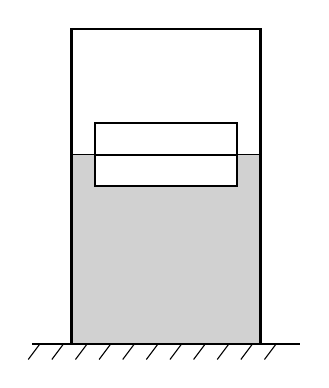
\begin{tikzpicture}[x=1cm,y=1cm]
\fill[black!18] (0,0) rectangle (2.4,2.4);
\draw[thick] (0,4)--(0,0)--(2.4,0)--(2.4,4)--cycle;
\draw (0,2.4)--(2.4,2.4);
\filldraw[fill=white,thick] (.3,2.0) rectangle (2.1,2.4);
\filldraw[fill=white,thick] (.3,2.4) rectangle (2.1,2.8);
\draw[thick] (-.5,0)--(2.9,0);
\foreach \x in {-.4,-.1,.2,.5,.8,1.1,1.4,1.7,2,2.3,2.6} \draw (\x,0)--++(-.15,-.2);
\end{tikzpicture}\end{center}
\begin{enumerate}
\item Если воду заменить на керосин, то глубина погружения брусков уменьшится.
\item Сила Архимеда, действующая на бруски, равна $20\,\text{Н}$.
\item Плотность материала, из которого изготовлены бруски, равна $500\,\text{кг}/\text{м}^{3}$.
\item Если на верхний брусок положить груз массой $0{,}7\,\text{кг}$, то бруски утонут.
\item Если в стопку добавить ещё два таких же бруска, то глубина её погружения увеличится на $10\,\text{см}$.
\end{enumerate}
}{
\smallskip\noindent\textbf{Решение от GPT}\par
$F_A=2mg=20\,\text{Н}$. Погружена половина суммарного объёма, поэтому $\rho_{\text{б}}=\rho_{\text{в}}/2=500\,\text{кг}/\text{м}^3$. В керосине погружение увеличится. Максимальная поддерживаемая масса $4\,\text{кг}$, поэтому груз $0{,}7\,\text{кг}$ не утопит систему. При добавлении ещё двух брусков погруженная толщина возрастёт с $5$ до $10\,\text{см}$, то есть на $5\,\text{см}$. Ответ: $23$.
}

% Source E74C4C: https://ege.fipi.ru/bank/questions.php?search=1&proj=BA1F39653304A5B041B656915DC36B38&qid=E74C4C
\BankTask{E74C4C}{
Учащиеся роняли с башни шарики для настольного тенниса и снимали их полёт цифровой видеокамерой. Обработка видеозаписей позволила построить графики зависимости пути $s$, пройденного шариком, и его скорости $v$ от времени падения $t$.
\begin{center}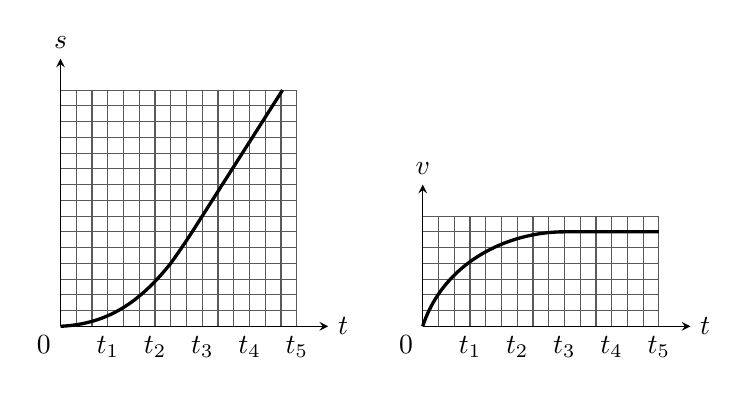
\begin{tikzpicture}[x=.2cm,y=.2cm,>=stealth]
\draw[thin,black!65,step=1] (0,0) grid (15,15);
\draw[->] (0,0)--(17,0) node[right] {$t$};\draw[->] (0,0)--(0,17) node[above] {$s$};
\node[below left] at (0,0) {$0$};
\foreach \x/\i in {3/1,6/2,9/3,12/4,15/5} \node[below] at (\x,0) {$t_{\i}$};
\draw[very thick] (0,0) .. controls (3,.15) and (5,1.5) .. (7,4) .. controls (8,5.4) and (8.49,6.2) .. (9,7) --(14.1,15);
\begin{scope}[xshift=4.6cm]
\draw[thin,black!65,step=1] (0,0) grid (15,7);
\draw[->] (0,0)--(17,0) node[right] {$t$};\draw[->] (0,0)--(0,9) node[above] {$v$};
\node[below left] at (0,0) {$0$};
\foreach \x/\i in {3/1,6/2,9/3,12/4,15/5} \node[below] at (\x,0) {$t_{\i}$};
\draw[very thick] (0,0) .. controls (1.3,4) and (5.3,6) .. (9,6) --(15,6);
\end{scope}\end{tikzpicture}\end{center}
\begin{enumerate}
\item В течение всего времени падения ($0$ — $t_{5}$) потенциальная энергия шарика в поле тяжести, отсчитываемая от основания башни, уменьшалась.
\item В течение всего времени падения ($0$ — $t_{5}$) величина импульса шарика постоянно возрастала.
\item Величина ускорения, с которым падал шарик, уменьшалась в интервале времени ($0$ — $t_{3}$).
\item Величина ускорения, с которым падал шарик, увеличивалась в интервале времени ($0$ — $t_{3}$) и оставалась постоянной при $t>t_{4}$.
\item Сумма кинетической и потенциальной энергий шарика оставалась неизменной во время падения.
\end{enumerate}
}{
\smallskip\noindent\textbf{Решение от GPT}\par
Шарик всё время опускается: $E_{\text{п}}=mgh$ уменьшается. Наклон графика $v(t)$ до $t_3$ уменьшается, значит ускорение уменьшается. Затем скорость и импульс постоянны. Сопротивление воздуха совершает отрицательную работу, поэтому механическая энергия не сохраняется. Ответ: $13$.
}

\end{document}
